%%%%%%%%%%%%%%%%%%%%%%%%%%%%%%%%%%%%%%%%%
% Jacobs Landscape Poster
% LaTeX Template
% Version 1.1 (14/06/14)
%
% Created by:
% Computational Physics and Biophysics Group, Jacobs University
% https://teamwork.jacobs-university.de:8443/confluence/display/CoPandBiG/LaTeX+Poster
% 
% Further modified by:
% Nathaniel Johnston (nathaniel@njohnston.ca)
%
% This template has been downloaded from:
% http://www.LaTeXTemplates.com
%
% License:
% CC BY-NC-SA 3.0 (http://creativecommons.org/licenses/by-nc-sa/3.0/)
%
%%%%%%%%%%%%%%%%%%%%%%%%%%%%%%%%%%%%%%%%%

%----------------------------------------------------------------------------------------
%	PACKAGES AND OTHER DOCUMENT CONFIGURATIONS
%----------------------------------------------------------------------------------------

\documentclass[final]{beamer}

\usepackage[scale=1.24]{beamerposter} % Use the beamerposter package for laying out the poster

\usetheme{confposter} % Use the confposter theme supplied with this template
\definecolor{mcgarnet}{rgb}{0.38, 0, 0.08}
\definecolor{mcgray}{rgb}{0.9, 0.9, 0.9}
\definecolor{mcorange}{rgb}{0.91,0.42,0.0}

\setbeamercolor{block title}{fg=mcgarnet,bg=white} % Colors of the block titles
\setbeamercolor{block body}{fg=black,bg=white} % Colors of the body of blocks
\setbeamercolor{block alerted title}{fg=mcgray,bg=mcgarnet} % Colors of the highlighted block titles
\setbeamercolor{title in headline}{fg=mcgarnet,bg=white}
\setbeamercolor{author in headline}{fg=black,bg=white}
\setbeamercolor{block alerted body}{fg=black,bg=mcgray} % Colors of the body of highlighted blocks
\setbeamercolor{cboxb}{fg=white,bg=mcgarnet}
\setbeamercolor{item}{fg=mcorange}
\setbeamercolor{item projected}{fg=white,bg=mcorange}
% Many more colors are available for use in beamerthemeconfposter.sty

%-----------------------------------------------------------
% Define the column widths and overall poster size
% To set effective sepwid, onecolwid and twocolwid values, first choose how many columns you want and how much separation you want between columns
% In this template, the separation width chosen is 0.024 of the paper width and a 4-column layout
% onecolwid should therefore be (1-(# of columns+1)*sepwid)/# of columns e.g. (1-(4+1)*0.024)/4 = 0.22
% Set twocolwid to be (2*onecolwid)+sepwid = 0.464
% Set threecolwid to be (3*onecolwid)+2*sepwid = 0.708

\newlength{\sepwid}
\newlength{\onecolwid}
\newlength{\twocolwid}
\newlength{\threecolwid}
\setlength{\paperwidth}{48in} % A0 width: 46.8in
\setlength{\paperheight}{36in} % A0 height: 33.1in
\setlength{\sepwid}{0.024\paperwidth} % Separation width (white space) between columns
\setlength{\onecolwid}{0.22\paperwidth} % Width of one column
\setlength{\twocolwid}{0.464\paperwidth} % Width of two columns
\setlength{\threecolwid}{0.708\paperwidth} % Width of three columns
\setlength{\topmargin}{-0.5in} % Reduce the top margin size
%-----------------------------------------------------------

\usepackage{graphicx}  % Required for including images

\usepackage{booktabs} % Top and bottom rules for tables

%----------------------------------------------------------------------------------------
%	TITLE SECTION 
%----------------------------------------------------------------------------------------

\title{HABPi -- A Cross-Discipline Hands-On Adventure} % Poster title

\author{Robert E. Lowe and Sarah M. Graham} % Author(s)

\institute{Maryville College and Pellissippi State Community College} % Institution(s)

%----------------------------------------------------------------------------------------

\begin{document}

\addtobeamertemplate{block end}{}{\vspace*{2ex}} % White space under blocks
\addtobeamertemplate{block alerted end}{}{\vspace*{2ex}} % White space under highlighted (alert) blocks

\setlength{\belowcaptionskip}{2ex} % White space under figures
\setlength\belowdisplayshortskip{2ex} % White space under equations

\begin{frame}[t] % The whole poster is enclosed in one beamer frame

\begin{columns}[t] % The whole poster consists of three major columns, the second of which is split into two columns twice - the [t] option aligns each column's content to the top

\begin{column}{\sepwid}\end{column} % Empty spacer column

\begin{column}{\onecolwid} % The first column

%----------------------------------------------------------------------------------------
%	OBJECTIVES
%----------------------------------------------------------------------------------------

\begin{alertblock}{Objectives}
HABPi is both an open source software development project and a project in STEM education.  Our goals are to:
\begin{itemize}
\item Provide a low cost general purpose hardware and software framework for High Altitude Ballooning~\cite{lowe}.
\item Introduce students of all ages to STEM activities and allow them to participate in research projects.
\item Conduct workshops and create materials to support teachers in HAB related activities.
\item Conduct professional high altitude research.
\end{itemize}
\end{alertblock}

%----------------------------------------------------------------------------------------
%	INTRODUCTION
%----------------------------------------------------------------------------------------

\begin{block}{Introduction}
One of the main problems facing STEM education in the United States is a lack of meaningful opportunities for STEM exploration~\cite{dejarnette}. 
Moreover, the current STEM climate requires a broad base of knowledge which is best obtained through project based learning~\cite{kennedy}.  HABPi is one such project which combines elements of engineering, science, computer science, mathematics, and data analysis.  All of this is wrapped in an unforgettable adventure which takes students to the edge of space!

\end{block}

%------------------------------------------------

\begin{figure}
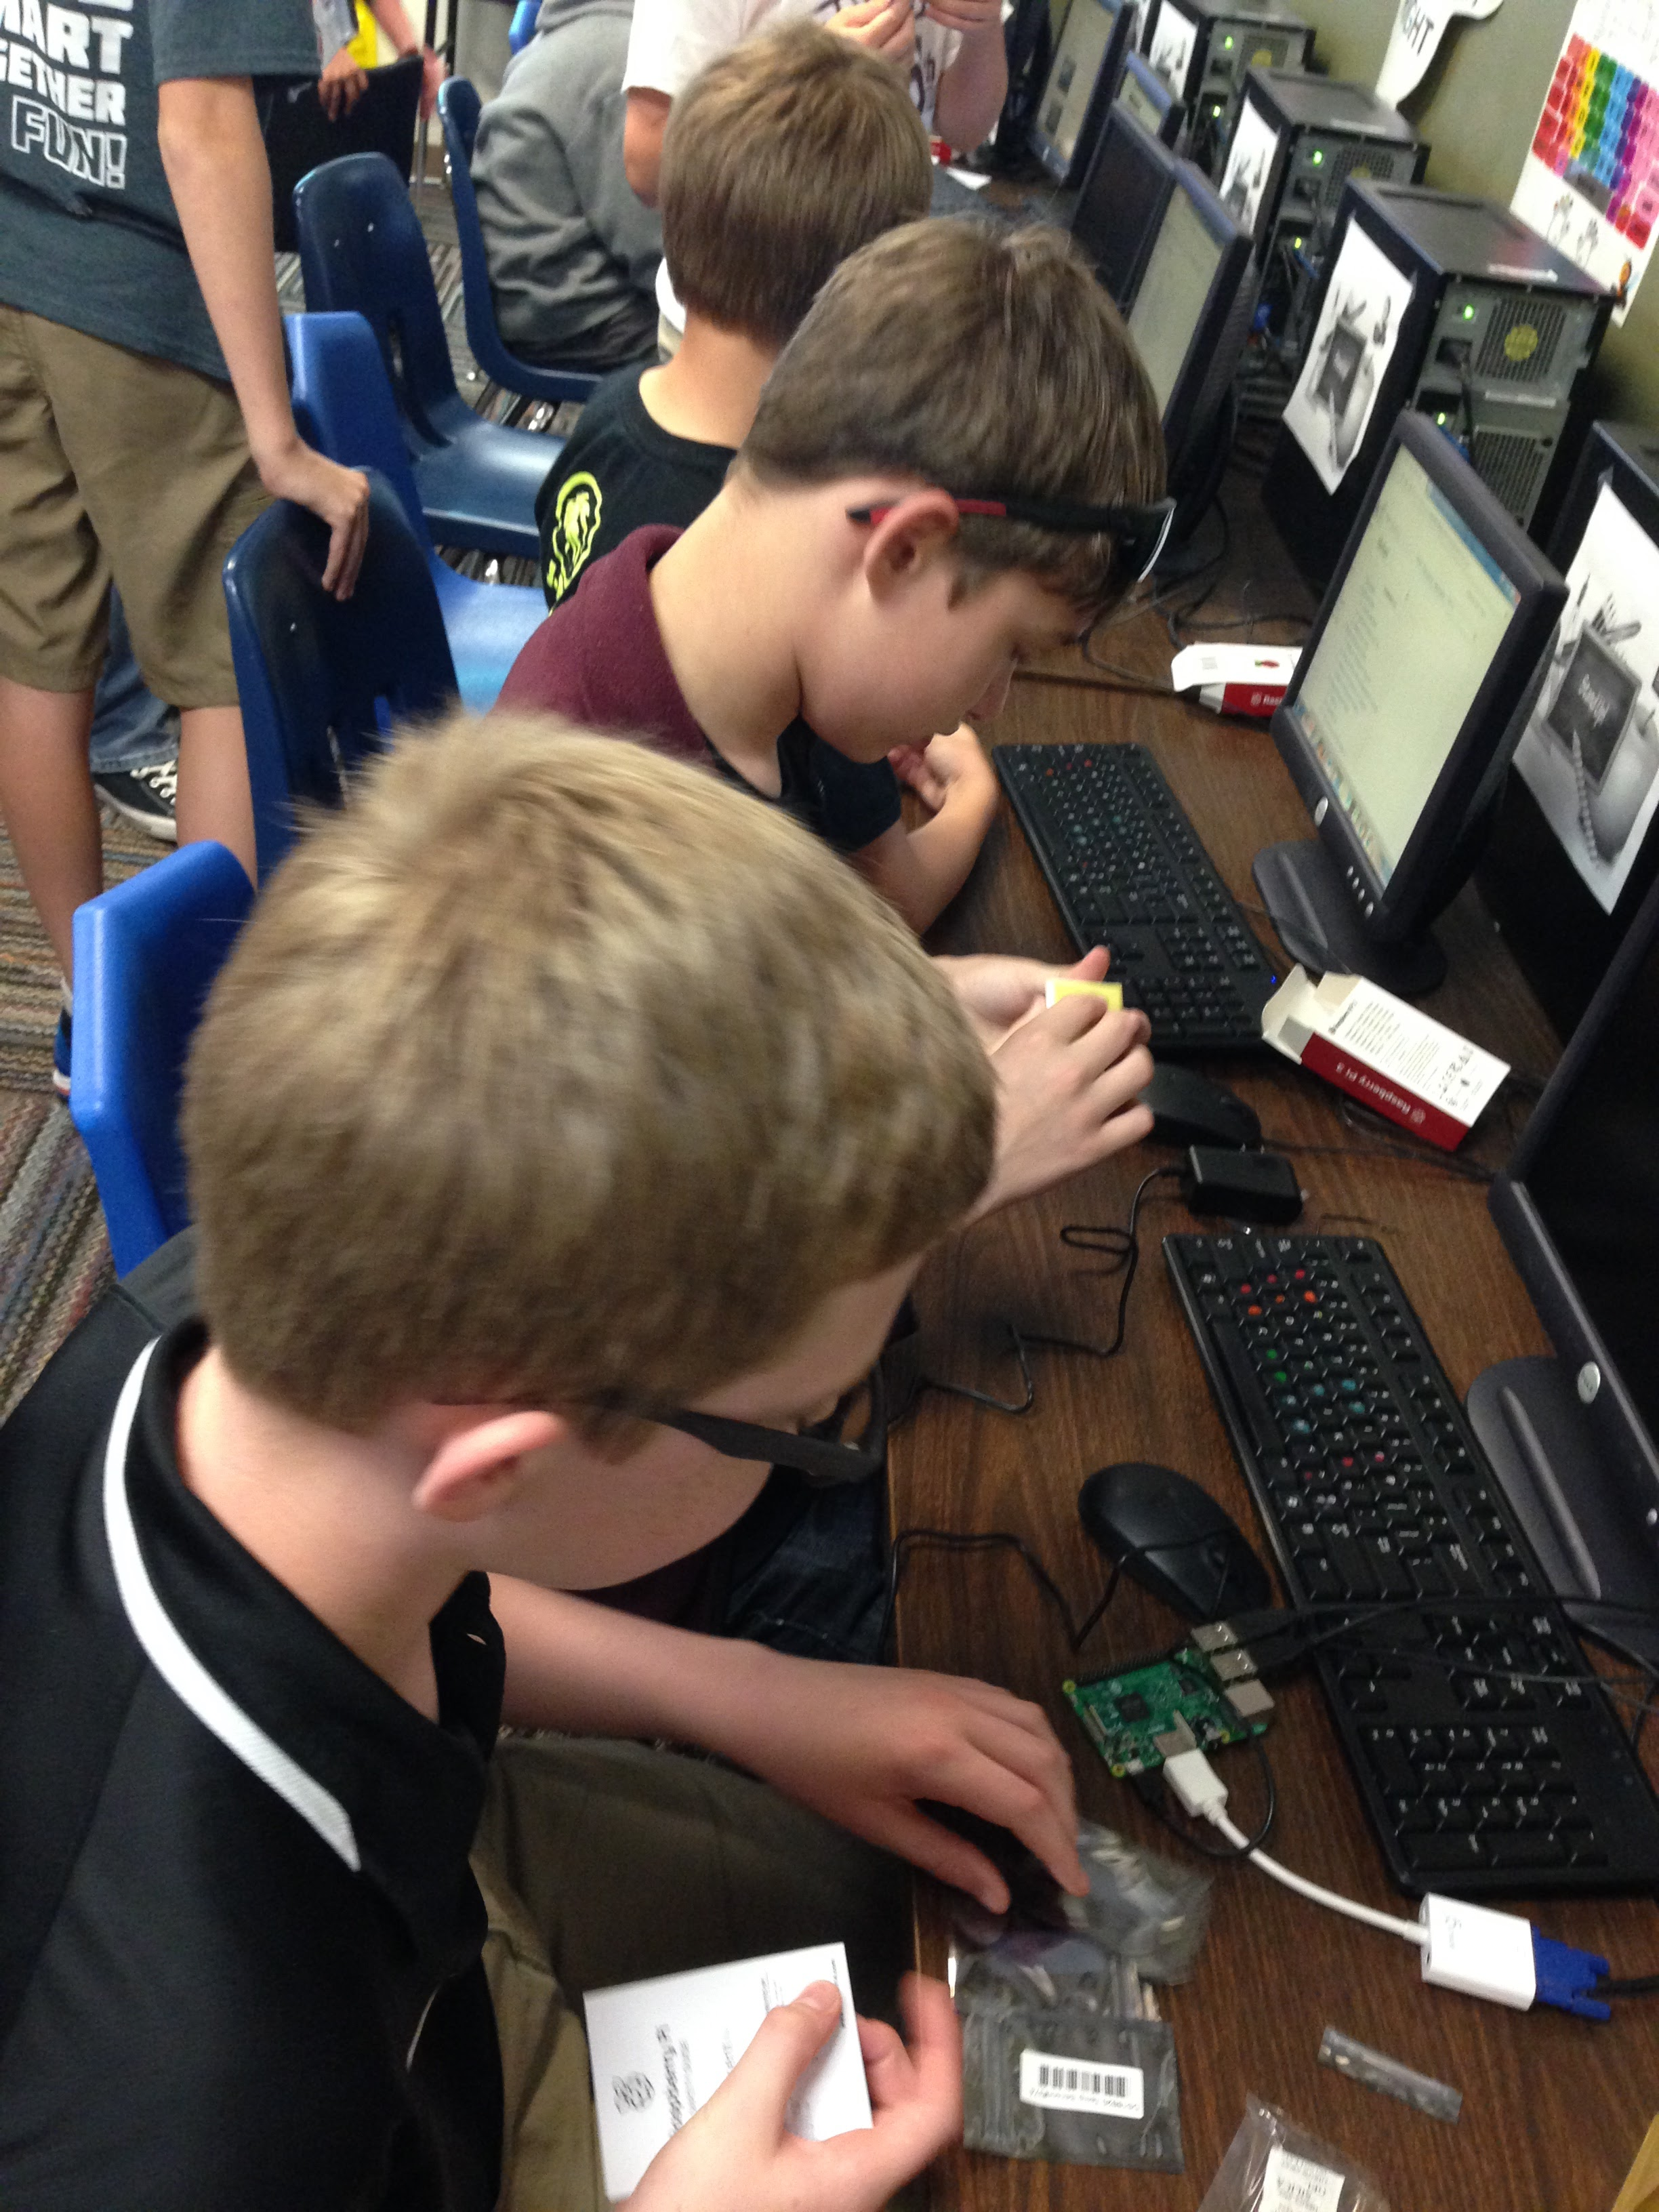
\includegraphics[width=0.6\linewidth]{CCS_Electronics}
\caption{Students Assemble Electronics}
\end{figure}

%----------------------------------------------------------------------------------------

\end{column} % End of the first column

\begin{column}{\sepwid}\end{column} % Empty spacer column

\begin{column}{\twocolwid} % Begin a column which is two columns wide (column 2)

%----------------------------------------------------------------------------------------
% Money Shot	
%----------------------------------------------------------------------------------------

\begin{figure}
    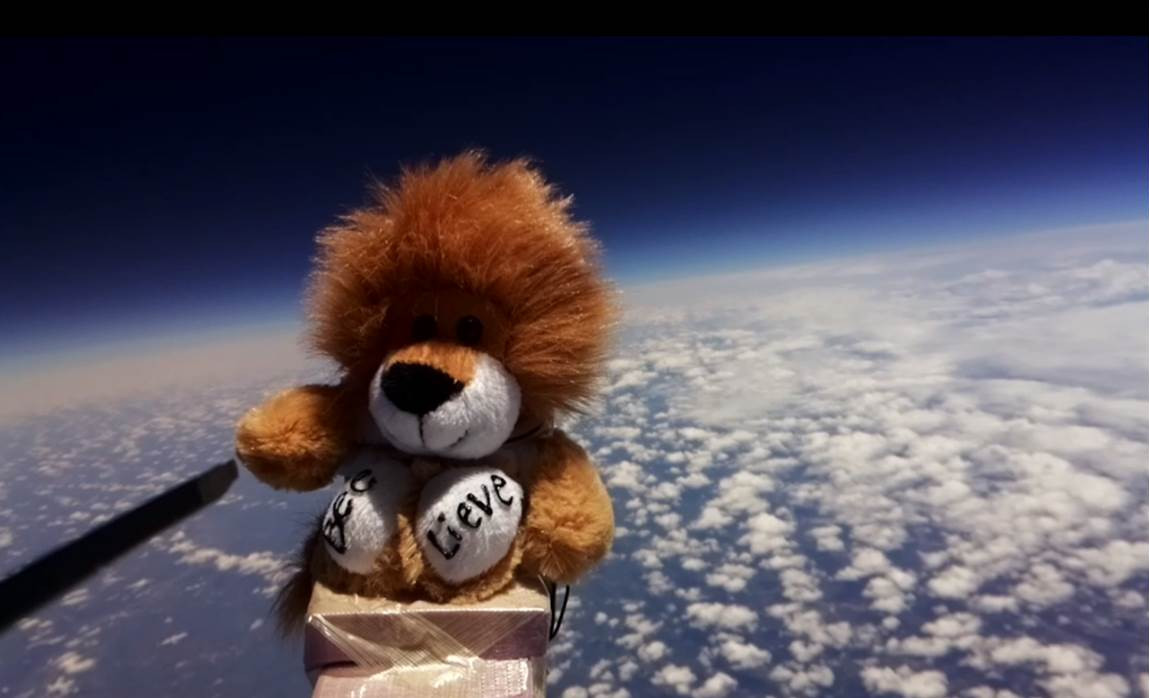
\includegraphics[width=0.8\linewidth]{lion}
    \caption{CCS Fifth Grade Payload at an altitude of 27 km - May 13, 2017}
\end{figure}

%----------------------------------------------------------------------------------------

\begin{columns}[t,totalwidth=\twocolwid] % Split up the two columns wide column again

\begin{column}{\onecolwid} % The first column within column 2 (column 2.1)

%----------------------------------------------------------------------------------------
% Launch
%----------------------------------------------------------------------------------------
\begin{figure}
   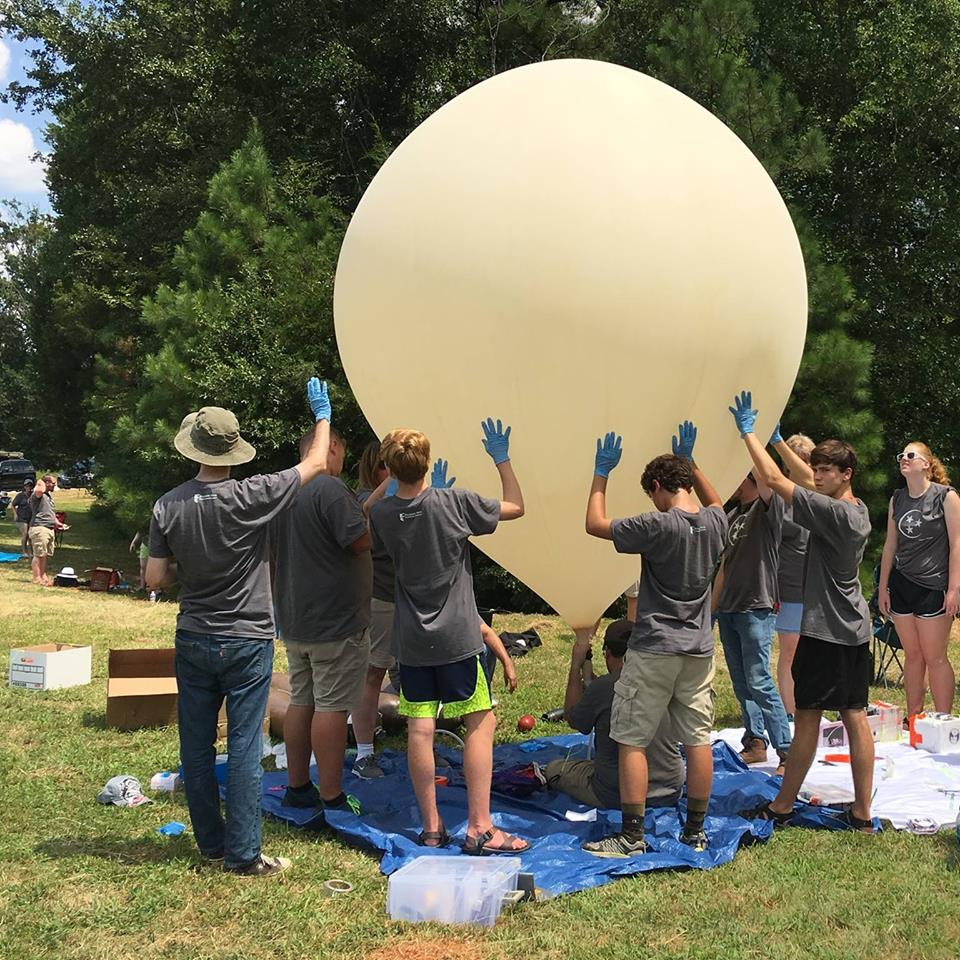
\includegraphics[width=0.6\linewidth]{launch1}
   \caption{Students Launch a Balloon}
\end{figure}
%----------------------------------------------------------------------------------------

%----------------------------------------------------------------------------------------
%	MATERIALS
%----------------------------------------------------------------------------------------

\begin{block}{Materials}

A HABPi expedition uses the following elements:

\begin{itemize}
\item Payload boxes, constructed of foam and tape.  These are designed and built by the students.
\item A Raspberry Pi computer
\item Sensors and Experiments (Designed, built, and programmed by students.)
\item A stratospheric research balloon, rigged and flown by students and HABPi team members.
\end{itemize}


\end{block}

%----------------------------------------------------------------------------------------


\end{column} % End of column 2.1

\begin{column}{\onecolwid} % The second column within column 2 (column 2.2)



%----------------------------------------------------------------------------------------
%	Learning Objectives
%----------------------------------------------------------------------------------------

\begin{block}{Learning Objectives}
\begin{description}
\item[Computer Science] Programming automated experiments and sensors.
\item[Structural Engineering] Construction of a box which can withstand extreme cold and low pressure environments all while working within strict weight requirements.
\item[Electrical Engineering] Construction of experiments and sensor arrays.
\item[Mathematics and Statistics] Collect and analyze real world data.
\end{description}
\end{block}

%----------------------------------------------------------------------------------------

%----------------------------------------------------------------------------------------
%	Data
%----------------------------------------------------------------------------------------
\begin{figure}
    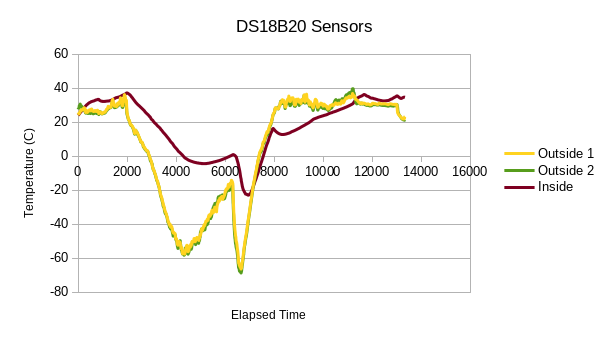
\includegraphics[width=0.8\linewidth]{ds18b20-data}
    \caption{Temperature Data Reveals Atmospheric Layers}
\end{figure}
%----------------------------------------------------------------------------------------



\end{column} % End of column 2.2

\end{columns} % End of the split of column 2

\end{column} % End of the second column

\begin{column}{\sepwid}\end{column} % Empty spacer column

\begin{column}{\onecolwid} % The third column

%----------------------------------------------------------------------------------------
%	Roadmap
%----------------------------------------------------------------------------------------

\begin{block}{Project Timeline}
\begin{description}
\item[2016] Construct and fly HABPi prototypes with college students.
\item[2017] Pilot flights with grade school students of various age groups.
\item[2018] Plan curriculum possibilities and begin developing classroom materials.
\item[2019] Finish classroom materials and manuals, conduct flights with more groups of students.
\item[Summer 2020] Begin workshops to train teachers in the use of HABPi materials in classrooms.
\end{description}

\end{block}
%----------------------------------------------------------------------------------------

%	REFERENCES
%----------------------------------------------------------------------------------------

\begin{block}{References}

\nocite{*} % Insert publications even if they are not cited in the poster
\small{\bibliographystyle{unsrt}
\bibliography{sources}\vspace{0.75in}}

\end{block}

%----------------------------------------------------------------------------------------
%	ACKNOWLEDGEMENTS
%----------------------------------------------------------------------------------------

%\setbeamercolor{block title}{fg=red,bg=white} % Change the block title color

\begin{block}{Acknowledgements}

\small{\rmfamily{We would like to thank Sherilyn Dawson from Concord Christian School and Gregg Vandergriff from Boy Scout Troop 255 for participating in the student pilot HAB flights. We would also like to thank NASA and ORAU for their financial support.}}

\end{block}

%----------------------------------------------------------------------------------------
%	CONTACT INFORMATION
%----------------------------------------------------------------------------------------

\setbeamercolor{block alerted title}{fg=mcgarnet,bg=mcorange} % Change the alert block title colors
\setbeamercolor{block alerted body}{fg=black,bg=mcgray} % Change the alert block body colors

\begin{alertblock}{Contact Information}

\begin{itemize}
\item Web: \href{http://www.github.com/habpi}{http://www.github.com/habpi}
\item Email: \href{mailto:robert.lowe@maryvillecollege.edu}{robert.lowe@maryvillecollege.edu}
\item Phone: +1 (865) 981-8169
\end{itemize}

\end{alertblock}

\begin{center}
\begin{tabular}{ccc}

\includegraphics[width=0.4\linewidth]{Maryville-College.jpg} & \hfill & 
\includegraphics[width=0.4\linewidth]{pstcc.png}
\end{tabular}
\end{center}

%----------------------------------------------------------------------------------------

\end{column} % End of the third column

\end{columns} % End of all the columns in the poster

\end{frame} % End of the enclosing frame

\end{document}
